\documentclass[12pt]{article}
\usepackage{amsmath}
\usepackage{amsfonts}
\usepackage{enumerate}
\usepackage{pgfplots}
\usepackage{calc}
\usepackage{graphicx}
\usepackage{float}
\usepackage{hyperref}
\usepackage{chngpage}
\pgfplotsset{compat=1.12}
\hypersetup{colorlinks,urlcolor=blue}
\graphicspath{{./code/src/}}
\begin{document}
\title{Computer Science M146, Homework 2}
\date{February 6th, 2018}
\author{Michael Wu\\UID: 404751542}
\maketitle

\section*{Problem 1}

\paragraph{a)}

We have the following points
\[
        \begin{array}{c c c}
                x_1 & x_2 & y\\
                \hline
                -1 & -1 & -1\\
                -1 & 1 & -1\\
                1 & -1 & -1\\
                1 & 1 & 1
        \end{array}
\]
Initializing \(\pmb{\theta}=\left<0,0\right>\) and \(b=0\) and running the perceptron algorithm on this list from top to bottom yields
\(\pmb{\theta}=\left<1,1\right>\) and \(b=-1\). Then
\[y=\begin{cases}
        1 & \text{if } \theta_1x_1+\theta_2x_2+b\geq0\\
        -1 & \text{if } \theta_1x_1+\theta_2x_2+b<0
\end{cases}\]
which separates our training data perfectly. This is not the only unique way to separate our data, as if we chose \(\pmb{\theta}=\left<2,1\right>\)
and \(b=-2\) this would be a valid perceptron as well.

\paragraph{b)}

We have the following points
\[
        \begin{array}{c c c}
                x_1 & x_2 & y\\
                \hline
                -1 & -1 & -1\\
                -1 & 1 & 1\\
                1 & -1 & 1\\
                1 & 1 & -1
        \end{array}
\]
No valid perceptron exists, because this data is not linearly separable.

\section*{Problem 2}

\paragraph{a)}

\begin{align*}
        \frac{\partial J(\pmb{\theta})}{\partial \theta_j}
        &=-\frac{\partial}{\partial \theta_j}\sum_{n=1}^N \left[y_n \ln\left(\frac{1}{1+e^{-\pmb{\theta}^T x_n}}\right)
        +(1-y_n)\ln\left(\frac{e^{-\pmb{\theta}^T x_n}}{1+e^{-\pmb{\theta}^T x_n}}\right)\right]\\
        &=-\frac{\partial}{\partial \theta_j}\sum_{n=1}^N \left[-y_n \ln\left(1+e^{-\pmb{\theta}^T x_n}\right)
        +(1-y_n)\left(-\pmb{\theta}^T x_n-\ln\left(1+e^{-\pmb{\theta}^T x_n}\right)\right)\right]\\
        &=-\sum_{n=1}^N \left[y_nx_{nj}\frac{e^{-\pmb{\theta}^T x_n }}{1+e^{-\pmb{\theta}^T x_n}}
        +(1-y_n)\left(-x_{nj}+x_{nj}\frac{e^{-\pmb{\theta}^T x_n }}{1+e^{-\pmb{\theta}^T x_n}}\right)\right]\\
        &=-\sum_{n=1}^N x_{nj}\left[y_n\frac{e^{-\pmb{\theta}^T x_n }}{1+e^{-\pmb{\theta}^T x_n}}
        +(1-y_n)\left(\frac{e^{-\pmb{\theta}^T x_n }}{1+e^{-\pmb{\theta}^T x_n}}-1\right)\right]\\
        &=-\sum_{n=1}^N x_{nj}\left[\frac{e^{-\pmb{\theta}^T x_n }}{1+e^{-\pmb{\theta}^T x_n}}+y_n-1\right]\\
        &=-\sum_{n=1}^N x_{nj}\left(y_n-\frac{1}{1+e^{-\pmb{\theta}^T x_n}}\right)\\
        &=\sum_{n=1}^N x_{nj}\left(h_{\pmb{\theta}}(x_n)-y_n\right)
\end{align*}

\section*{Problem 3}

\paragraph{a)}

\[\nabla J(\theta_0,\theta_1)=2\sum_{n=1}^N \left[w_n(\theta_0+\theta_1x_{n,1}-y_n)\left<1, x_{n,1}\right>\right]\]

\paragraph{b)}

First we will write out the partial derivative with respect to \(\theta_0\) and set it to zero.

\begin{align*}
        \frac{\partial J}{\partial \theta_0}=2\sum_{n=1}^N \left[w_n(\theta_0+\theta_1x_{n,1}-y_n)\right]&=0\\
        \sum_{n=1}^N \left[w_n(\theta_0+\theta_1x_{n,1}-y_n)\right]&=0\\
        \theta_0\sum_{n=1}^N w_n + \theta_1\sum_{n=1}^N w_nx_{n,1} - \sum_{n=1}^N w_ny_n&=0\\
        a\theta_0 + b\theta_1 &= c
\end{align*}
where \(a=\sum_{n=1}^N w_n\), \(b=\sum_{n=1}^N w_nx_{n,1}\), and \(c=\sum_{n=1}^N w_ny_n\). Next we
will write out the partial derivative with respect to \(\theta_1\) and set it to zero.
\begin{align*}
        \frac{\partial J}{\partial \theta_1}=2\sum_{n=1}^N \left[x_{n,1}w_n(\theta_0+\theta_1x_{n,1}-y_n)\right]&=0\\
        \sum_{n=1}^N \left[x_{n,1}w_n(\theta_0+\theta_1x_{n,1}-y_n)\right]&=0\\
        \theta_0\sum_{n=1}^N x_{n,1}w_n + \theta_1\sum_{n=1}^N w_nx_{n,1}^2 - \sum_{n=1}^N x_{n,1}w_ny_n&=0\\
        b\theta_0 + d\theta_1 &= e
\end{align*}
where \(d=\sum_{n=1}^N w_nx_{n,1}^2\) and \(e=\sum_{n=1}^N x_{n,1}w_ny_n\). Then solving this system of equations gives
\begin{align*}
        \theta_0&=\frac{e-d\theta_1}{b}\\
        \frac{a}{b}(e-d\theta_1)+b\theta_1&=c\\
        \frac{ae}{b}+\left(b-\frac{ad}{b}\right)\theta_1&=c\\
        \frac{b^2-ad}{b}\theta_1&=c-\frac{ae}{b}\\
        \theta_1&=\frac{bc-ae}{b^2-ad}
\end{align*}
\begin{align*}
        \theta_0&=\frac{e-d\frac{bc-ae}{b^2-ad}}{b}\\
        \theta_0&=\frac{eb^2-ade-bcd+ade}{b^3-abd}\\
        \theta_0&=\frac{eb-cd}{b^2-ad}
\end{align*}
Then we have a minimum at
\[(\theta_0,\theta_1)=\frac{1}{b^2-ad}\left<eb-cd, bc-ae\right>\]

\section*{Problem 4}

\paragraph{a)}

Assume that our data set is finite, so we have for all \((x_i,y_i)\in D\) there exists a \(w\) and \(\theta\) such that
\[y_i(w^Tx_i+\theta)>l\]
where \(l\) is the margin between our separating line and the closest point in our data set. Then we can multiply our
weight vector \(w\) and our threshold value \(\theta\) by \(\frac{1}{l}\) to get
\[y_i\left(\frac{1}{l}w^Tx_i+\frac{\theta}{l}\right)>1\]
Thus we can find a weight vector and threshold value that creates an optimal solution to the linear program with \(\delta=0\).

\paragraph{b)}

If we have an optimal solution to the linear problem, we have
\[y_i\left(w^Tx_i+\theta\right)>1\]
for all \((x_i,y_i)\in D\). In order for this to happen, \(y_i\) must always have the same sign as \(w^Tx_i+\theta\). Thus
\[y_i=\begin{cases}
        1 & \text{if }w^Tx_i+\theta\geq 0\\
        -1 & \text{if }w^Tx_i+\theta<0
\end{cases}\]
for all \((x_i,y_i)\in D\), and so \(D\) is linearly separable.

\paragraph{c)}

If \(0<\delta<1\), then our data set is linearly separable, using the same argument as above. Otherwise we cannot say anything about
if our data set is linearly separable.

\paragraph{d)}

An optimal solution is \(w=0\) and \(\theta=0\). Then
\[y_i(w^Tx_i+\theta)\geq 0\]
for any data set. The problem with this is that our resulting linear separator tells us nothing about our data set, as everything is
zero.

\paragraph{e)}

A possible optimal solution is \(w=\left<1,1,1\right>\) and \(\theta=0\).

\section*{Problem 5}

\paragraph{a)}

The data seems to be negatively correlated, with most points in the bottom right and top left. I believe
linear regression will do a relatively good job of fitting the data.

\begin{figure}[H]
        \begin{center}
                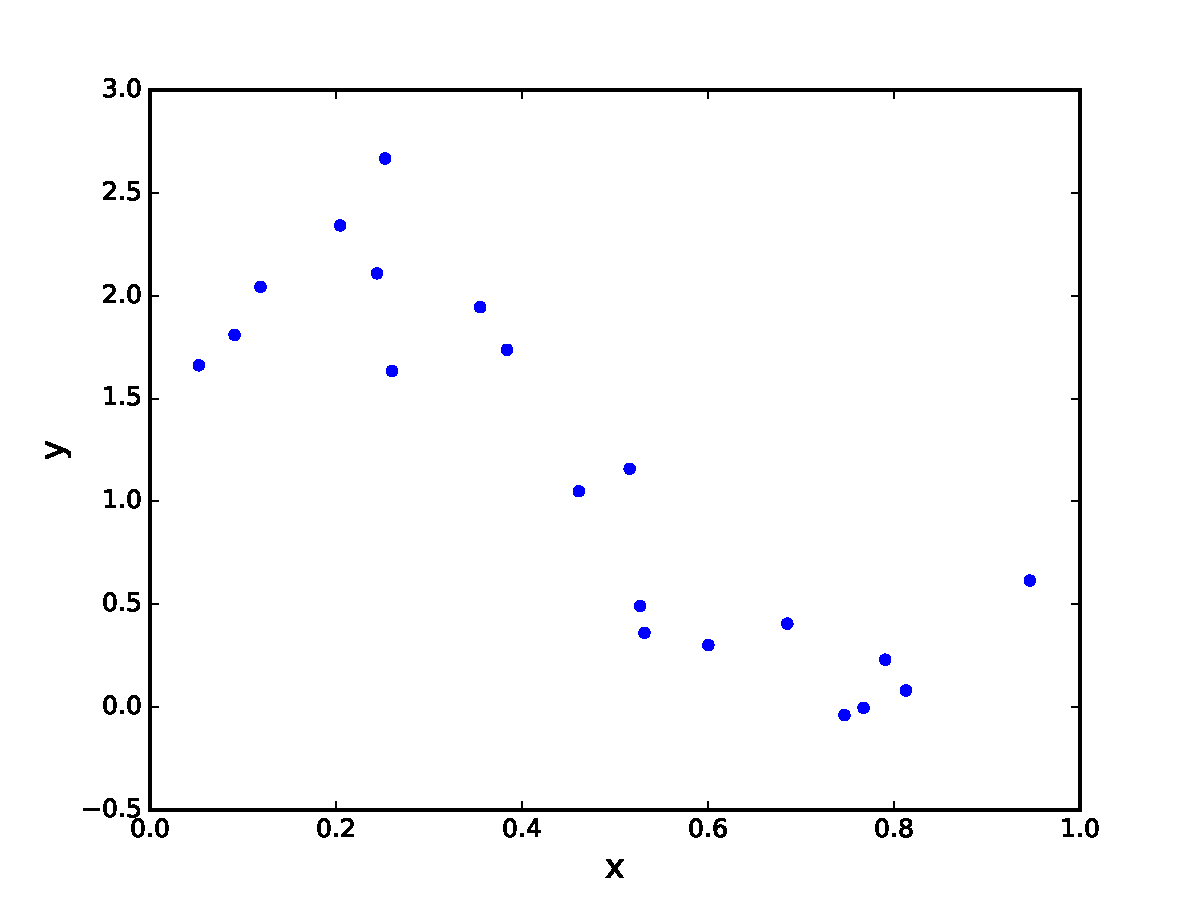
\includegraphics[height=2.5in]{trainData}
                \caption{Plot of training data.}
        \end{center}
\end{figure}

\begin{figure}[H]
        \begin{center}
                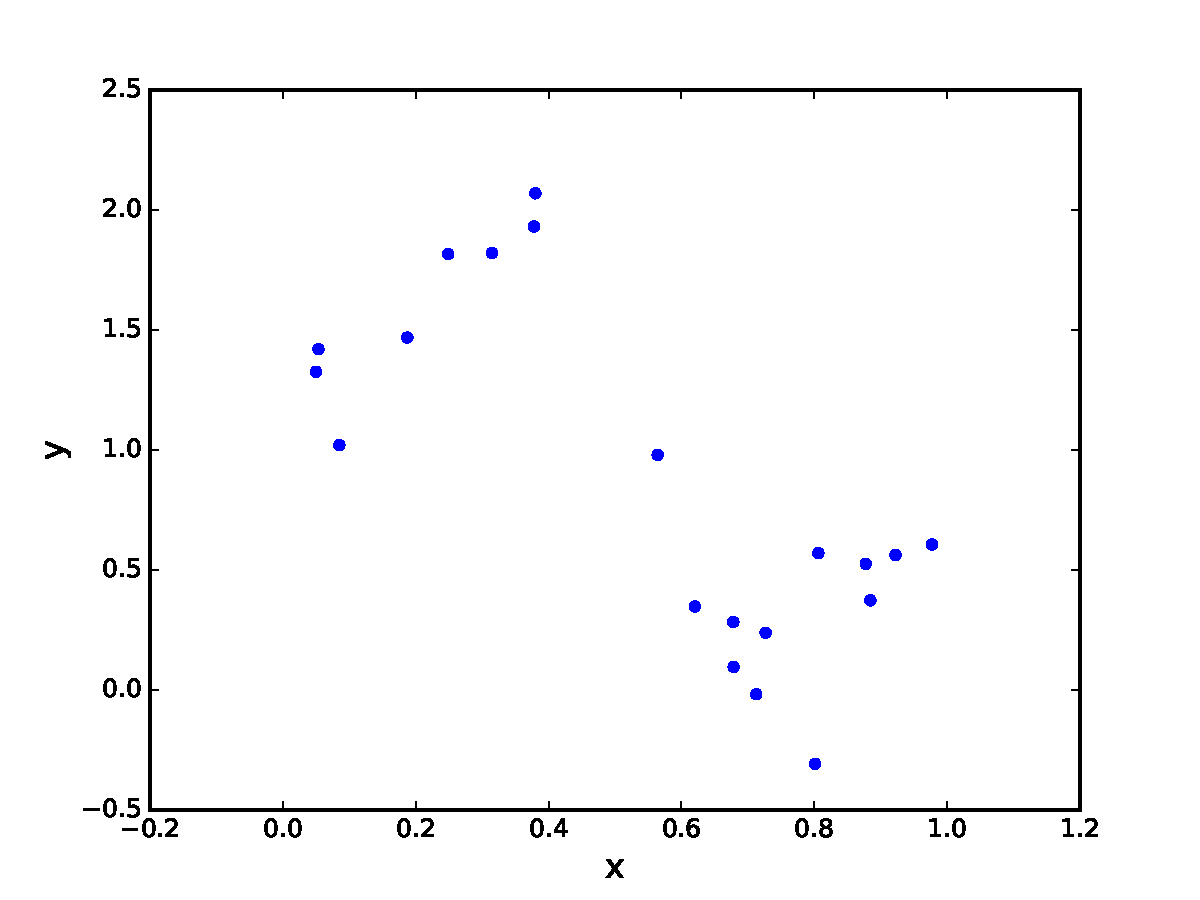
\includegraphics[height=2.5in]{testData}
                \caption{Plot of testing data.}
        \end{center}
\end{figure}

\paragraph{b)}

I implemented this using the following code

\begin{verbatim}
m = self.m_
Phi = np.zeros((n,m+1))
for i in range(0,n):
    val=[1]
    index=[(m+1)*i]
    for j in range(0,m):
        val.append(val[j]*X.flat[i])
        index.append(index[j]+1)
    np.put(Phi, index, val)

return Phi
\end{verbatim}
This took care of creating feature vectors for linear regression as well as polynomial regression.

\paragraph{c)}

I simply computed the dot product of each feature vector with the weights in order to make a prediction for \(y\).

\paragraph{d)}

The results of the different \(\eta\) values are as follows.
\[
        \begin{array}{c | c c c c c}
                \eta & \theta_0 & \theta_1 & \text{Iterations} & J(\theta) & \text{Runtime}\\
                \hline
                0.0001 & 2.2704 & -2.4606 & 10000 & 4.0863 & 1.060399\\
                0.001 & 2.4464 & -2.8163 & 7021 & 3.9125 & 0.794983\\
                0.01 & 2.4464 & -2.8163 & 765 & 3.9125 & 0.079679\\
                0.0407 & -9.40*10^{18}& -4.65*10^{18} & 10000 & 2.71*10^{39} & 1.042172\\
                \frac{1}{1+k} & 2.4464 & -2.8163 & 1357 & 3.9125 & 0.142043\\
                \text{Closed Form} & 2.4464 & -2.8163 & \text{N/A} & 3.9125 & 0.000560\\
        \end{array}
\]
The larger step sizes converged quicker, until \(\eta=0.0407\) when the step size became too large.

\paragraph{e)}

The closed form solution is
\[\theta=\left(\mathbf{X}^T\mathbf{X}\right)^{-1}\mathbf{X}^T\mathbf{y}\]
The coefficients obtained match the ones obtained with gradient descent, though the runtime was about two to four orders of magnitude
faster.

\paragraph{f)}

It took \(1357\) iterations and \(0.142043\) seconds for our algorithm with our proposed learning rate to converge.

\paragraph{g)}

I already implemented this in part b.

\paragraph{h)}

We use RMSE because \(J(\theta)\) increases with more training data, which we do not want because it makes it harder to judge how accurate our
fit is. RMSE is an average. Additionally, \(J(\theta)\) scales with the square of our error, so we want to take the square root in order to make
our error scale more linearly.

\paragraph{i)}

The polynomial of degree \(m=5\) best fits our data, with the smallest test RMSE of \(0.355137742884\). There is evidence of underfitting
on the left of the plot, because both training and testing errors are higher there. There is evidence of overfitting on the right, as our
training error decreases and our test error increases there.

\begin{figure}[H]
        \begin{center}
                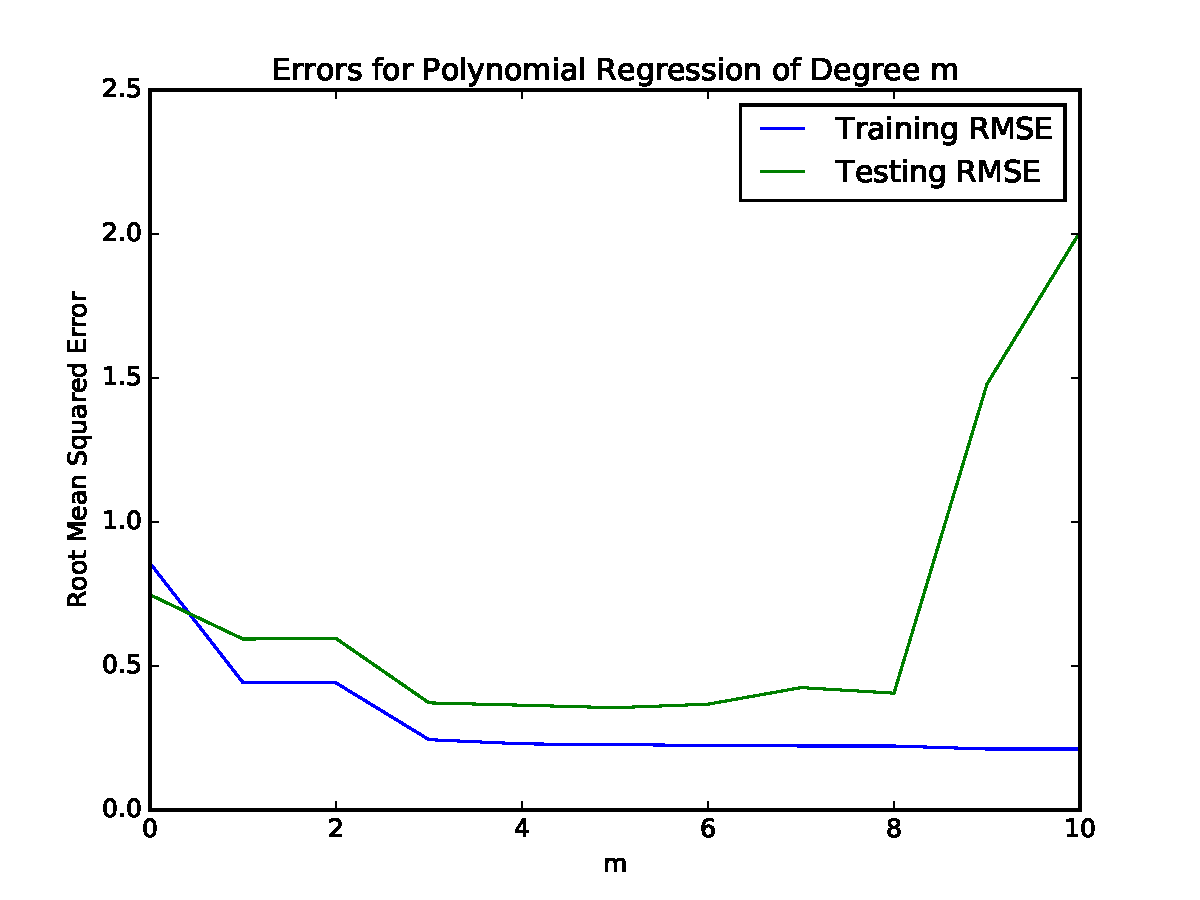
\includegraphics[height=2.5in]{polynomialRegression}
                \caption{Plot of how well polynomial regressions of varying degrees fits our data.}
        \end{center}
\end{figure}

\end{document}